Our architecture for implementing security metrics is straight forward. We declare a \textit{base security metric} type from which all metrics inherit three capabilities: 
\begin{itemize}
\item Check Prerequisites: is invoked either directly by the caller or in the metric's own calculate method to ensure all items necessary for the calculation are present.
\item Calculate: returns the resulting measurement
\item Get Metadata: returns the environment and ancillary data used during the calculation. 
\end{itemize}
 
\begin{minipage}{.45\linewidth}
\begin{figure}[H]

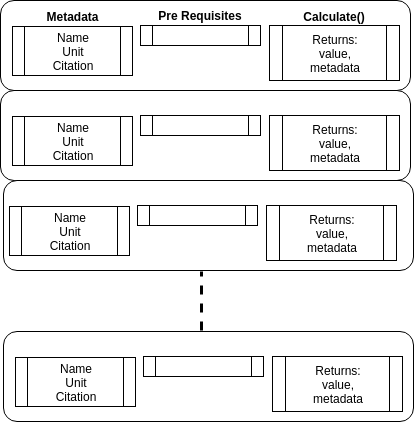
\includegraphics[width=.7\linewidth]{img/SecMet_archs.png}
\caption{Security Metric Catalog (\textbf{SecMet})}
\label{fig:automation:metric_arch}
\end{figure} 
\end{minipage}

As shown in Figure \ref{fig:automation:metric_arch}, this design allows us to implement a library of security metrics with a standard, stateless interface. 


% \begin{table}[ht]
% \caption{Implemented Metrics}
% \resizebox{.45\textwidth}{!}{%
% \begin{tabular}{@{}lp{.35\linewidth}l@{}}
% \toprule
% Metric Class & Description & Common Measurements \\ \midrule
% Structural & Metrics based on the structure of the attack graph; used to identify attributes like shortest path, mean path length, or total number of paths. & SP, NP, MPL \\
% Time-Based & Metrics that quantify time expectations for attributes like compromise, recovery, or incident response. & MTTF, MTTB, MTTR \\
% Probability-Based & Metrics that associate probabilities attack paths to quantify the security of the network. & NR, PP, EPL \\
% Temporal & Metrics that examine  vulnerability age on the system. & TAG \\ \bottomrule
% \end{tabular}%
% }
% \label{tab:metric_summary}
% \end{table}


\begin{figure}
      % \centering
        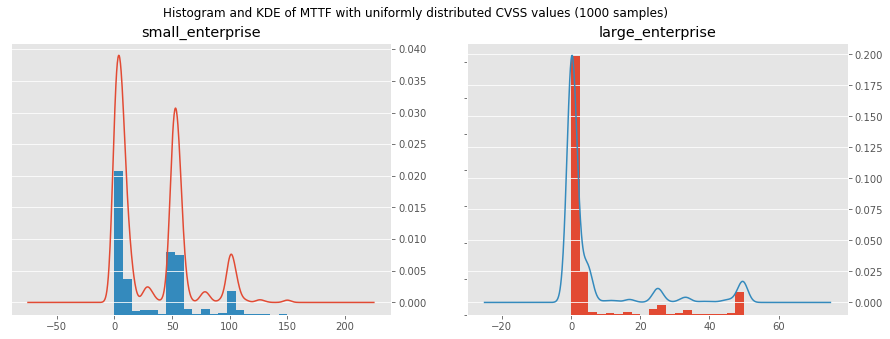
\includegraphics[width=\linewidth]{img/analysis/hist_kde_svl.png} 
        \caption{MTTF distributions over 1000 random CVSS score assignments (uniform-dist)\cite{Dacier_1994}} 
        \label{fig:mttf_score_distributions}
\end{figure}

\begin{figure}
      % \centering
        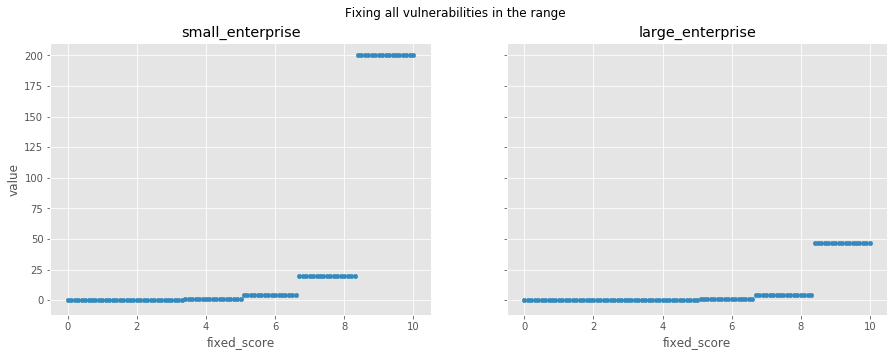
\includegraphics[width=\linewidth]{img/analysis/fixed_100.png} 
        \caption{Fixing all vulnerability scores to determine lower and upper bounds for metric}     \label{fig:score_map_stepping}
\end{figure}


% \begin{figure*}
%       % \centering
%         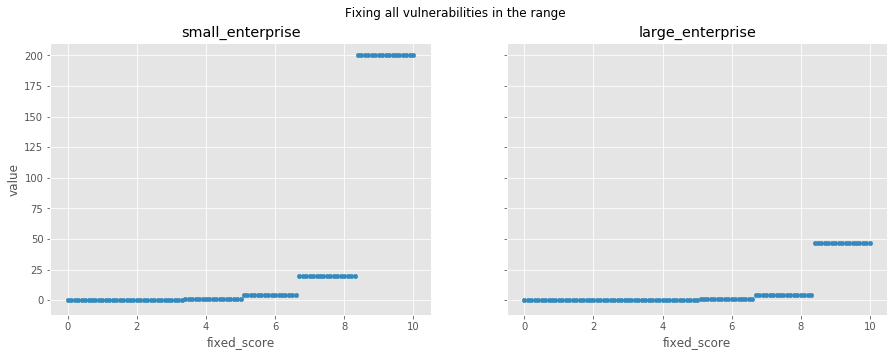
\includegraphics[width=\linewidth]{img/analysis/fixed_100.png} 
%         \caption{Fixing all vulnerability scores to determine lower and upper bounds for metric}     \label{fig:result_density}
% \end{figure*} 


% \begin{figure*}
%     \centering
%     \begin{subfigure}[t]{0.3\textwidth}
%         % \centering
%         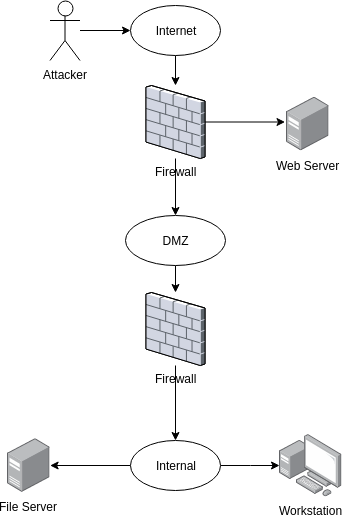
\includegraphics[width=\linewidth]{img/net_small.png} 
%         \caption{Small-sized network\cite{Ou_Appel_2005}} 
%         \label{fig:refnet_small}
%     \end{subfigure}
%           \begin{subfigure}[t]{0.3\textwidth}
%         \centering
%         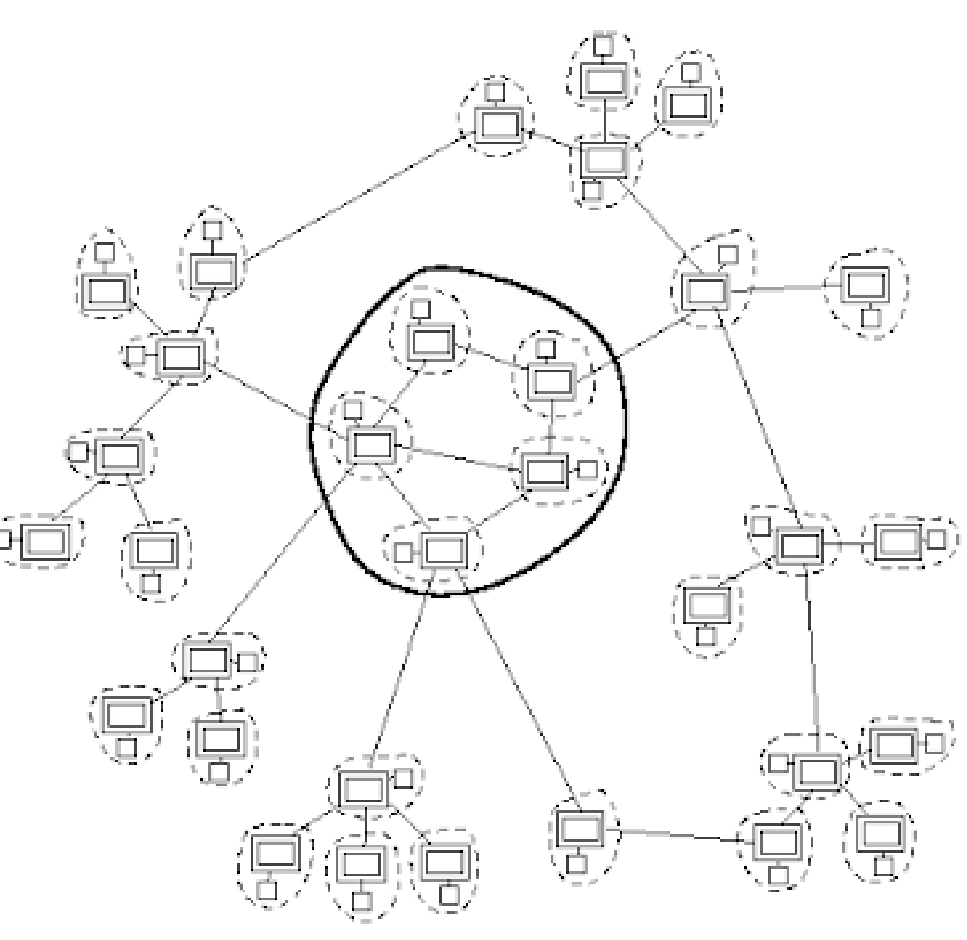
\includegraphics[width=\linewidth]{img/net_med_2.png}
%         \caption{Medium-sized network\cite{Cowie_Ogielski_Nicol_2002}}
%         \label{fig:refnet_med}
%     \end{subfigure}
%      \begin{subfigure}[t]{0.3\textwidth}
%         \centering
%         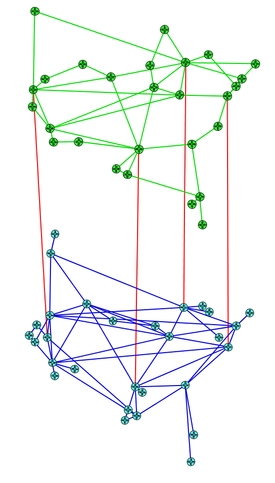
\includegraphics[width=\linewidth]{img/net_large.png}
%         \caption{Large-sized  network\cite{Cowie_Ogielski_Nicol_2002}}
%         \label{fig:refnet_large}
%     \end{subfigure}
%     \hfill
%     \caption{Different Sized Reference Networks}
%     \label{fig:refnets}
% \end{figure*}